
\chapter{Related Work}\label{ch:Ch.2}

This chapter surveys previous work in wildlife strike risk-index estimation and the state of the art Machine Learning techniques used for the proposed model development.

\section{Introduction to BRI\textsubscript{2}}
The second version of the Birdstrike Risk Index ($BRI_2$) is a sensitive tool that provides different time scale results allowing appropriate management planning and describes an airport-specific risk, based upon the historical trend of wildlife observations, in order to identify critical periods during the year.
Therefore, the index isn’t meant to be a prognostic index although it can be applied to assess specific theoretical risk scenarios \cite{soldatini2011wildlife}. 
Actually the $BRI_2$ algorithm is the standard adopted by ENAC.

The idea of $BRI_2$ is based on several factors, including bird biology and ecology, the association of different bird species with similar characteristics, group factor in Table \ref{tab-bird_species}, and the birdstrike event history, meaning the number of birdstrikes (and relative effects on flight, in Table \ref{tab-EOF}) recorded for the species in the particular airports (birdstrike factor). 
The “birdstrike factor” summarises an airport-specific evaluation of the danger of each species.
Since bird weight and flock size are of critical importance to the magnitude of a birdstrike event, average weights corresponding to each group of species were calculated based on Cramp and Simmons \cite{cramp1992handbook}.
In addition, the average daily number of flights per month has been included in the index.

\begin{table}
	\centering
	\scalebox{0.62}{
	\begin{tabular}{@{}ccc@{}}
		\toprule
		ID group & Species group & Some examples \\	\midrule
		1& Grebes and divers & Tachybaptus ruficollis, Podiceps nigricollis, Gavia immer \\
		2&  Cormorant, pelicans, swans and geese & Phalacrocorax carbo, Cignus olor, Anser anser \\
		3& Herons, storks, flamingoes & Ardea cinerea, Casmerodius albus \\
		4&  Ducks, pheasants, rallids & Anas platyrhynchos, Tadorna tadorna, Phasianus colchicus \\
		5& Birds of prey – large & Buteo buteo, Circus aeruginosus \\
		6& Birds of prey – small & Falco peregrinus, Falco tinnunculus \\
		7& Seabirds – large & Larus michahellis, Larus argentatus \\
		8& Seabirds – small & Chroicocephalus ridibundus, Sterna hirundo \\
		9& Waders & Charadrius alexandrinus, Recurvirostra avosetta, Tringa totanus \\
		10& Doves & Columba livia, Streptopelia decaocto \\
		11& Owls & Athene noctua, Tyto alba \\
		12& Swifts and swallows & Apus apus, Hirundo rustica \\
		13& Corvids & Corvus cornix, Pica pica \\
		14&  Non-flocking passerines and bats & Erithacus rubecula, Motacilla alba, Turdus merula, Nyctalus noctula \\
		15& Flocking passerines & Sturnus vulgaris\\
		16& Small mammals (,10 kg) & Vulpes vulpes \\
		17&  Large mammals (.10 kg) & Dama dama\\		\bottomrule
	\end{tabular}}
	\caption{. Distribution of bird species among different groups, based on species-specific ecological patterns (habitat, diet), body size, and social behavior (flocking vs. non flocking species). This distribution of species is the core of the formulation of the $BRI_2$.}
	\label{tab-bird_species}
\end{table}

\begin{table}
	\centering
	\scalebox{0.85}{
	\begin{tabular}{@{}ccc@{}}
		\toprule
		EOF Value & Category & Description \\	\midrule
		1 & None & None \\
		2 & Minor & Delay \\
		3 & Substantial & Precautionary landing, aborted take-off \\
		4 &  Serious & Engine(s) shutdown, forced landing, vision obscured \\
		5 & Catastrophice & Damage sustained makes it inadvisable to restore aircraft \\	\bottomrule
	\end{tabular}}
	\caption{Categories of the Effect On Flight (EOF) provoked by wildlife strike events.}
	\label{tab-EOF}
\end{table}

\section{Machine Learning overview}
The classic diagram of the programming concept is well represented on the left in Figure \ref{ML_programming}: the programmer sets the machine so that it performs an $f$ function that for each input provides the desired output.
The Machine Learning approach is different: the programmer sets the machine in the following way so that it is itself that determines which function $f$ (taken from a set of possible functions $H$ said Hypothesis Space) to use on data. The Figure  \ref{ML_programming} (on the right) shows what has been said (actually in the particular case of supervised learning, as explained below).

There are in fact three types of approach in Machine Learning:

\begin{itemize}
\item Supervised Learning: there is a strong distinction between input (features) as images and output (labels). The machine is trained ($f$ is defined) on a set of data labelled with the respective output (train-set) and can therefore subsequently be used on new input data never seen before.

\item Unsupervised Learning: there is no input data information, the machine must find patterns on the data; examples of unsupervised learning tasks are clustering or anomaly detection.

\item Reinforcement Learning: supervision is provided at a later stage (information is given on the consequences of decisions already taken). Note that here, unlike the other two cases, the time characterisation of the input is strong.
\end{itemize}

\begin{figure}
    \centering
    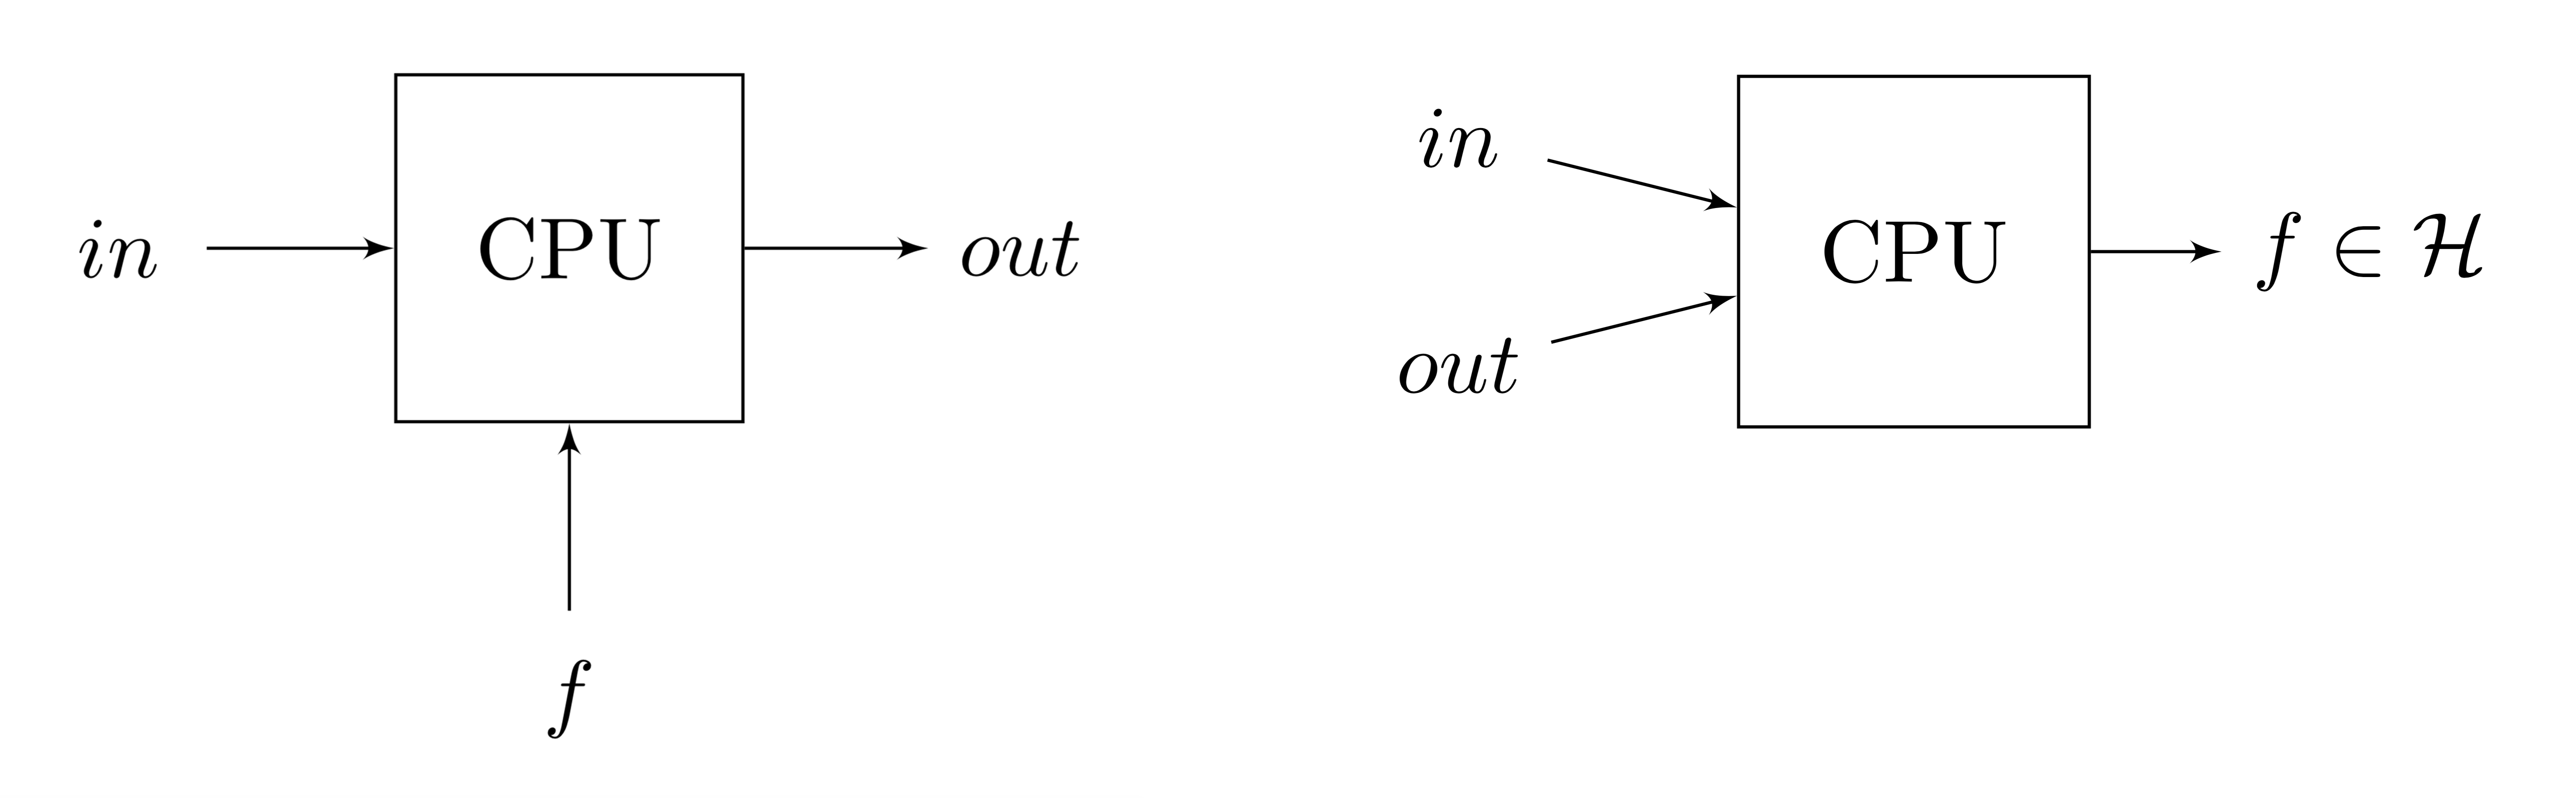
\includegraphics[width=14cm]{img/ml.png}
    \caption{Conceptual comparison of the classic programming approach compared to the one introduced by Machine Learning. On right is shown the classic programming, on left the Machine Learning approach.}\label{ML_programming}
\end{figure}

Machine Learning enables us to perform tasks that are too difficult to solve with fixed programs written and designed by human beings. From a scientific and philosophical point of view, Machine Learning is interesting because developing our understanding of it entails developing our understanding of the principles that underlie intelligence. In this relatively formal definition of the word "task", the process of learning itself is not the task. Learning is our means of attaining the ability to perform the task. Machine Learning tasks are usually described in terms of how the Machine Learning system should process an example. An example is a collection of features that have been quantitatively measured from an object or event that we want the Machine Learning system to process. We typically represent an example as a vector $x\in \mathbb{R}  ^n$ where each entry $x_i$ of the vector is another feature. For example, the features of an image are usually the values of the pixels in the image \cite{deeplearningbook}.

Many kinds of tasks can be solved with Machine Learning. Some of the most common Machine Learning tasks include classification, regression, denoising, anomaly detection. In particular regression was the task to be solved for this thesis work.

In this type of task, the machine is asked to predict a numerical value given some input. To solve this task, the learning algorithm is asked to output a function $f: \mathbb{R} \to \mathbb{R}^n$. This type of task is similar to classification, except that the format of output is different. An example of a regression task is the prediction of the expected claim amount that an insured person will make (used to set insurance premiums), or the prediction of future prices of securities. These kinds of predictions are also used for algorithmic trading.

\section{Deep Learning and Neural networks}\label{deep}
Neural networks, also called feedforward neural networks, or Multi Layer Perceptrons (MLPs), are the quintessential Deep Learning models. The goal of a neural network is to approximate the function $f^\star$. For example, for a classifier, $y=f^\star (x)$ maps an input $x$ to a category $y$. A neural network defines a mapping $y=f(x,\theta)$ and learns the value of the parameters $\theta$ that result in the best function approximation. These models are called feed forward because information flows through the function being evaluated from $x$, through the intermediate computations used to define $f$, and finally to the output $y$. There are no feedback connections in which outputs of the model are fed back into itself. When feedforward neural networks are extended to include feedback connections, they are called  recurrent neural networks which we will discuss in \ref{RNN}.

Feedforward neural networks are called networks because they are typically represented by composing together many different functions. The model is associated with a directed acyclic graph describing how the functions are composed together. 

\begin{figure}
	\centering
	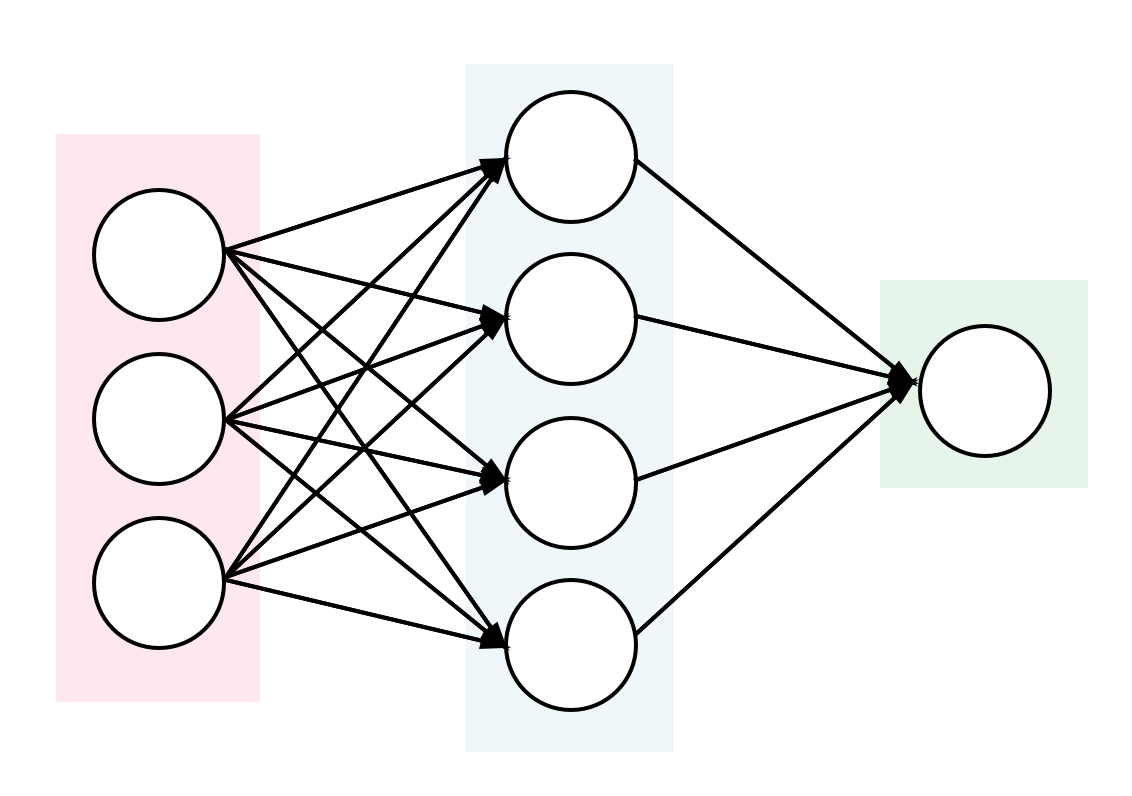
\includegraphics[width=8cm]{img/Single_Hidden_Network.png}
	\caption{The architecture of a single hidden layer network is composed of (from the left) the input layer that receives the data, the hidden layer, and finally the output layer.}
	\label{neuralnetwork}
\end{figure}

With a Single Hidden Layer Neural Network, in Figure \ref{neuralnetwork}, it is possible to approximate any function  $f: \mathbb{R}^n \to \mathbb{R}$, provided that there are enough hidden units (neurons in the intermediate layer between the input and output) \cite{cybenko1989approximation}.
The hidden layer name comes from the fact that the training data does not show the desired output for each of these layers. Adding additional hidden layers to the neural network we begin to talk about a deep network.

\subsection{Recurrent Neural Networks (RNNs)}\label{RNN}
In the previous section we considered feedforward neural networks whose connections did not form cycles. If we relax this condition, and allow cyclical connections as well, we obtain recurrent neural networks, Figure \ref{RNN_fig}, (RNNs). As with feedforward networks, many varieties of RNN have been proposed, such as Elman networks \cite{elman1990finding}, Jordan networks \cite{pollack1990recursive}, time delay neural networks \cite{lang1990time} and echo state networks \cite{jaeger2001echo}.

RNNs, are a family of neural networks for processing sequential data and sequences of values like $x^{(1)}, . . . , x^{(k)}$.
While the difference between a multilayer perceptron and an RNN may seem trivial, the implications for sequence learning are far-reaching. An MLP can only map from input to output vectors, whereas an RNN can, in principle, map from the entire history of previous inputs to each output. Indeed, the equivalent result to the universal approximation theory for MLPs is that an RNN with a sufficient number of hidden units can approximate any measurable sequence to sequence mapping to arbitrary accuracy \cite{hammer2000approximation}. The key point is that the recurrent connections allow a "memory" of previous inputs to persist in the network’s internal state, and thereby influence the network output\cite{graves2012supervised}.

\begin{figure}
	\centering
	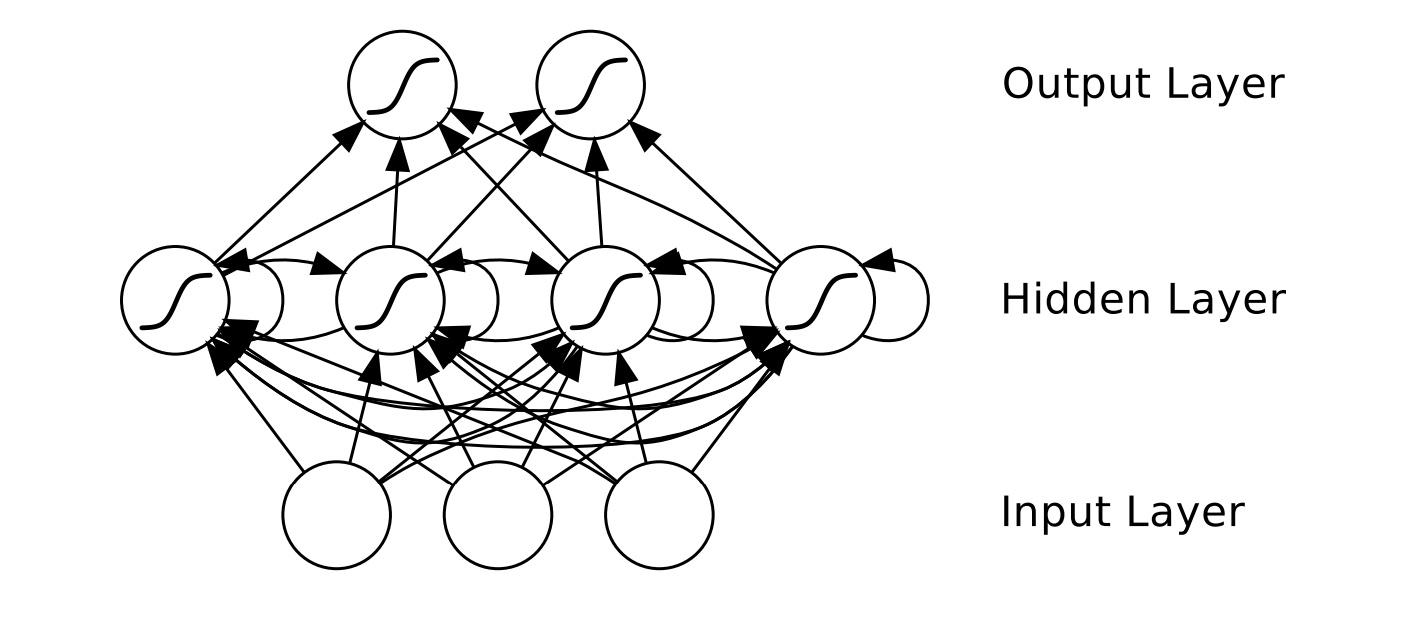
\includegraphics[width=11cm]{img/RNN.png}
	\caption{A recurrent neural network. The figure shown the recurrent connections whose forms cycles, relaxing the condition of feedforward networks.}
	\label{RNN_fig}
\end{figure}

\subsection{Long Short-Term Memory (LSTM)}\label{LSTM_subs}
The LSTM \cite{hochreiter1997long} architecture consists of a set of recurrently connected subnets, known as memory blocks. These blocks can be thought of as a differentiable version of the memory chips in a digital computer. Each block contains one or more self-connected memory cell and three multiplicative units: the input, output and forget gates, that provide continuous analogues of write, read and reset operations for the cells.

\begin{figure}
	\centering
	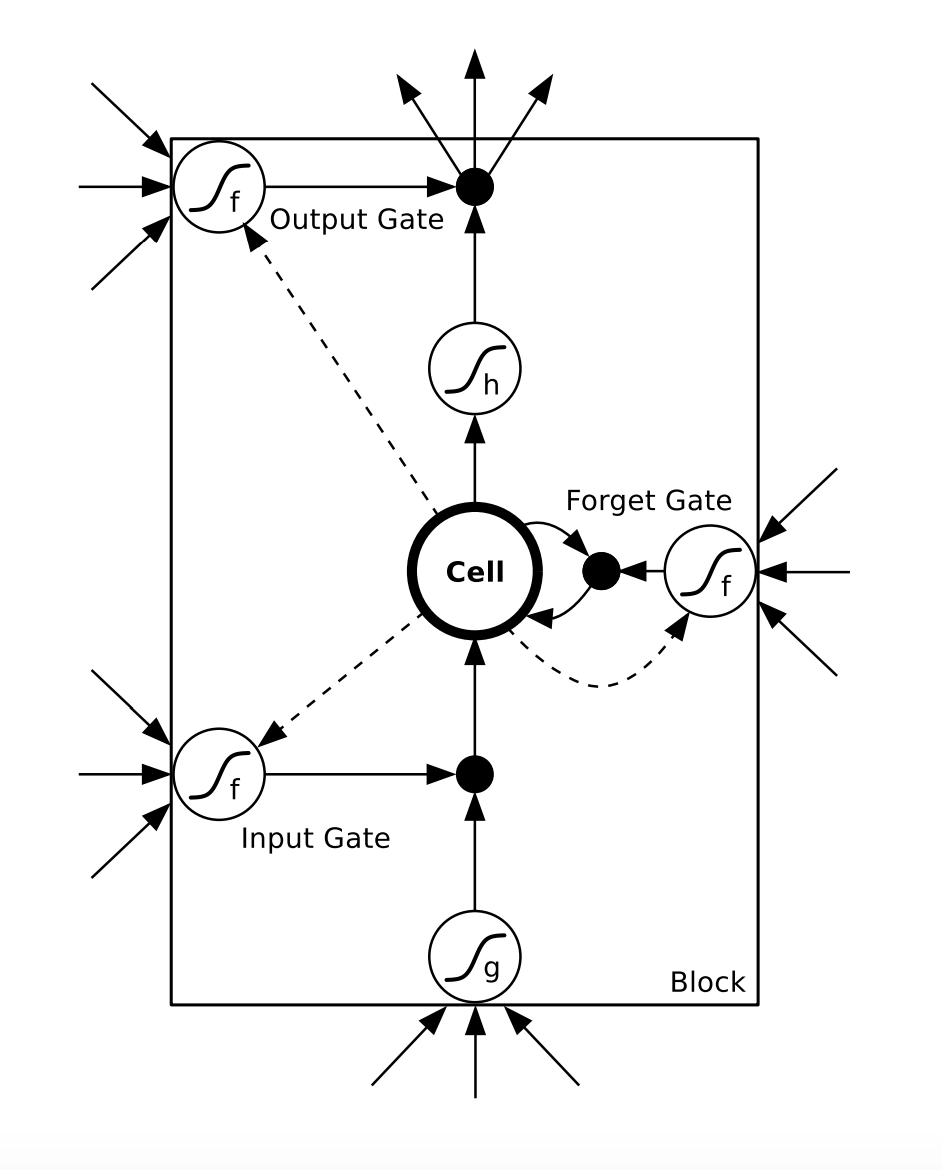
\includegraphics[width=6cm]{img/LSTM_block.png}
	\caption{LSTM memory block with one cell. The three gates are nonlinear summation units that collect activations from inside and outside the block, and control the activation of the cell via multiplications (small black circles). The input and output gates multiply the input and output of the cell while the forget gate multiplies the cell’s previous state. No activation function is applied within the cell. The gate activation function ‘f’ is usually the logistic sigmoid, so that the gate activations are between 0 (gate closed) and 1 (gate open). The cell input and output activation functions (‘g’ and ‘h’) are usually tanh or logistic sigmoid, though in some cases ‘h’ is the identity function.}
	\label{LSTM_block}
\end{figure}

Figure \ref{LSTM_block} provides an illustration of an LSTM memory block with a single cell.
The three gates are nonlinear summation units that collect activations from inside and outside the block, and control the activation of the cell via multiplications (small black circles).
The input and output gates multiply the input and output of the cell while the forget gate multiplies the cell’s previous state. No activation function is applied within the cell. The gate activation function $f$ is usually the logistic sigmoid, so that the gate activations are between 0 (gate closed) and 1 (gate open). The cell input and output activation functions ($g$ and $h$) are usually tanh or logistic sigmoid, though in some cases $h$ is the identity function.
An LSTM network is the same as a standard RNN, except that the summation units in the hidden layer are replaced by memory blocks, as illustrated in Figure \ref{LSTM}. LSTM blocks can also be mixed with ordinary summation units, although this is typically not necessary. The same output layers can be used for LSTM networks as for standard RNNs \cite{graves2012supervised}.

\begin{figure}
	\centering
	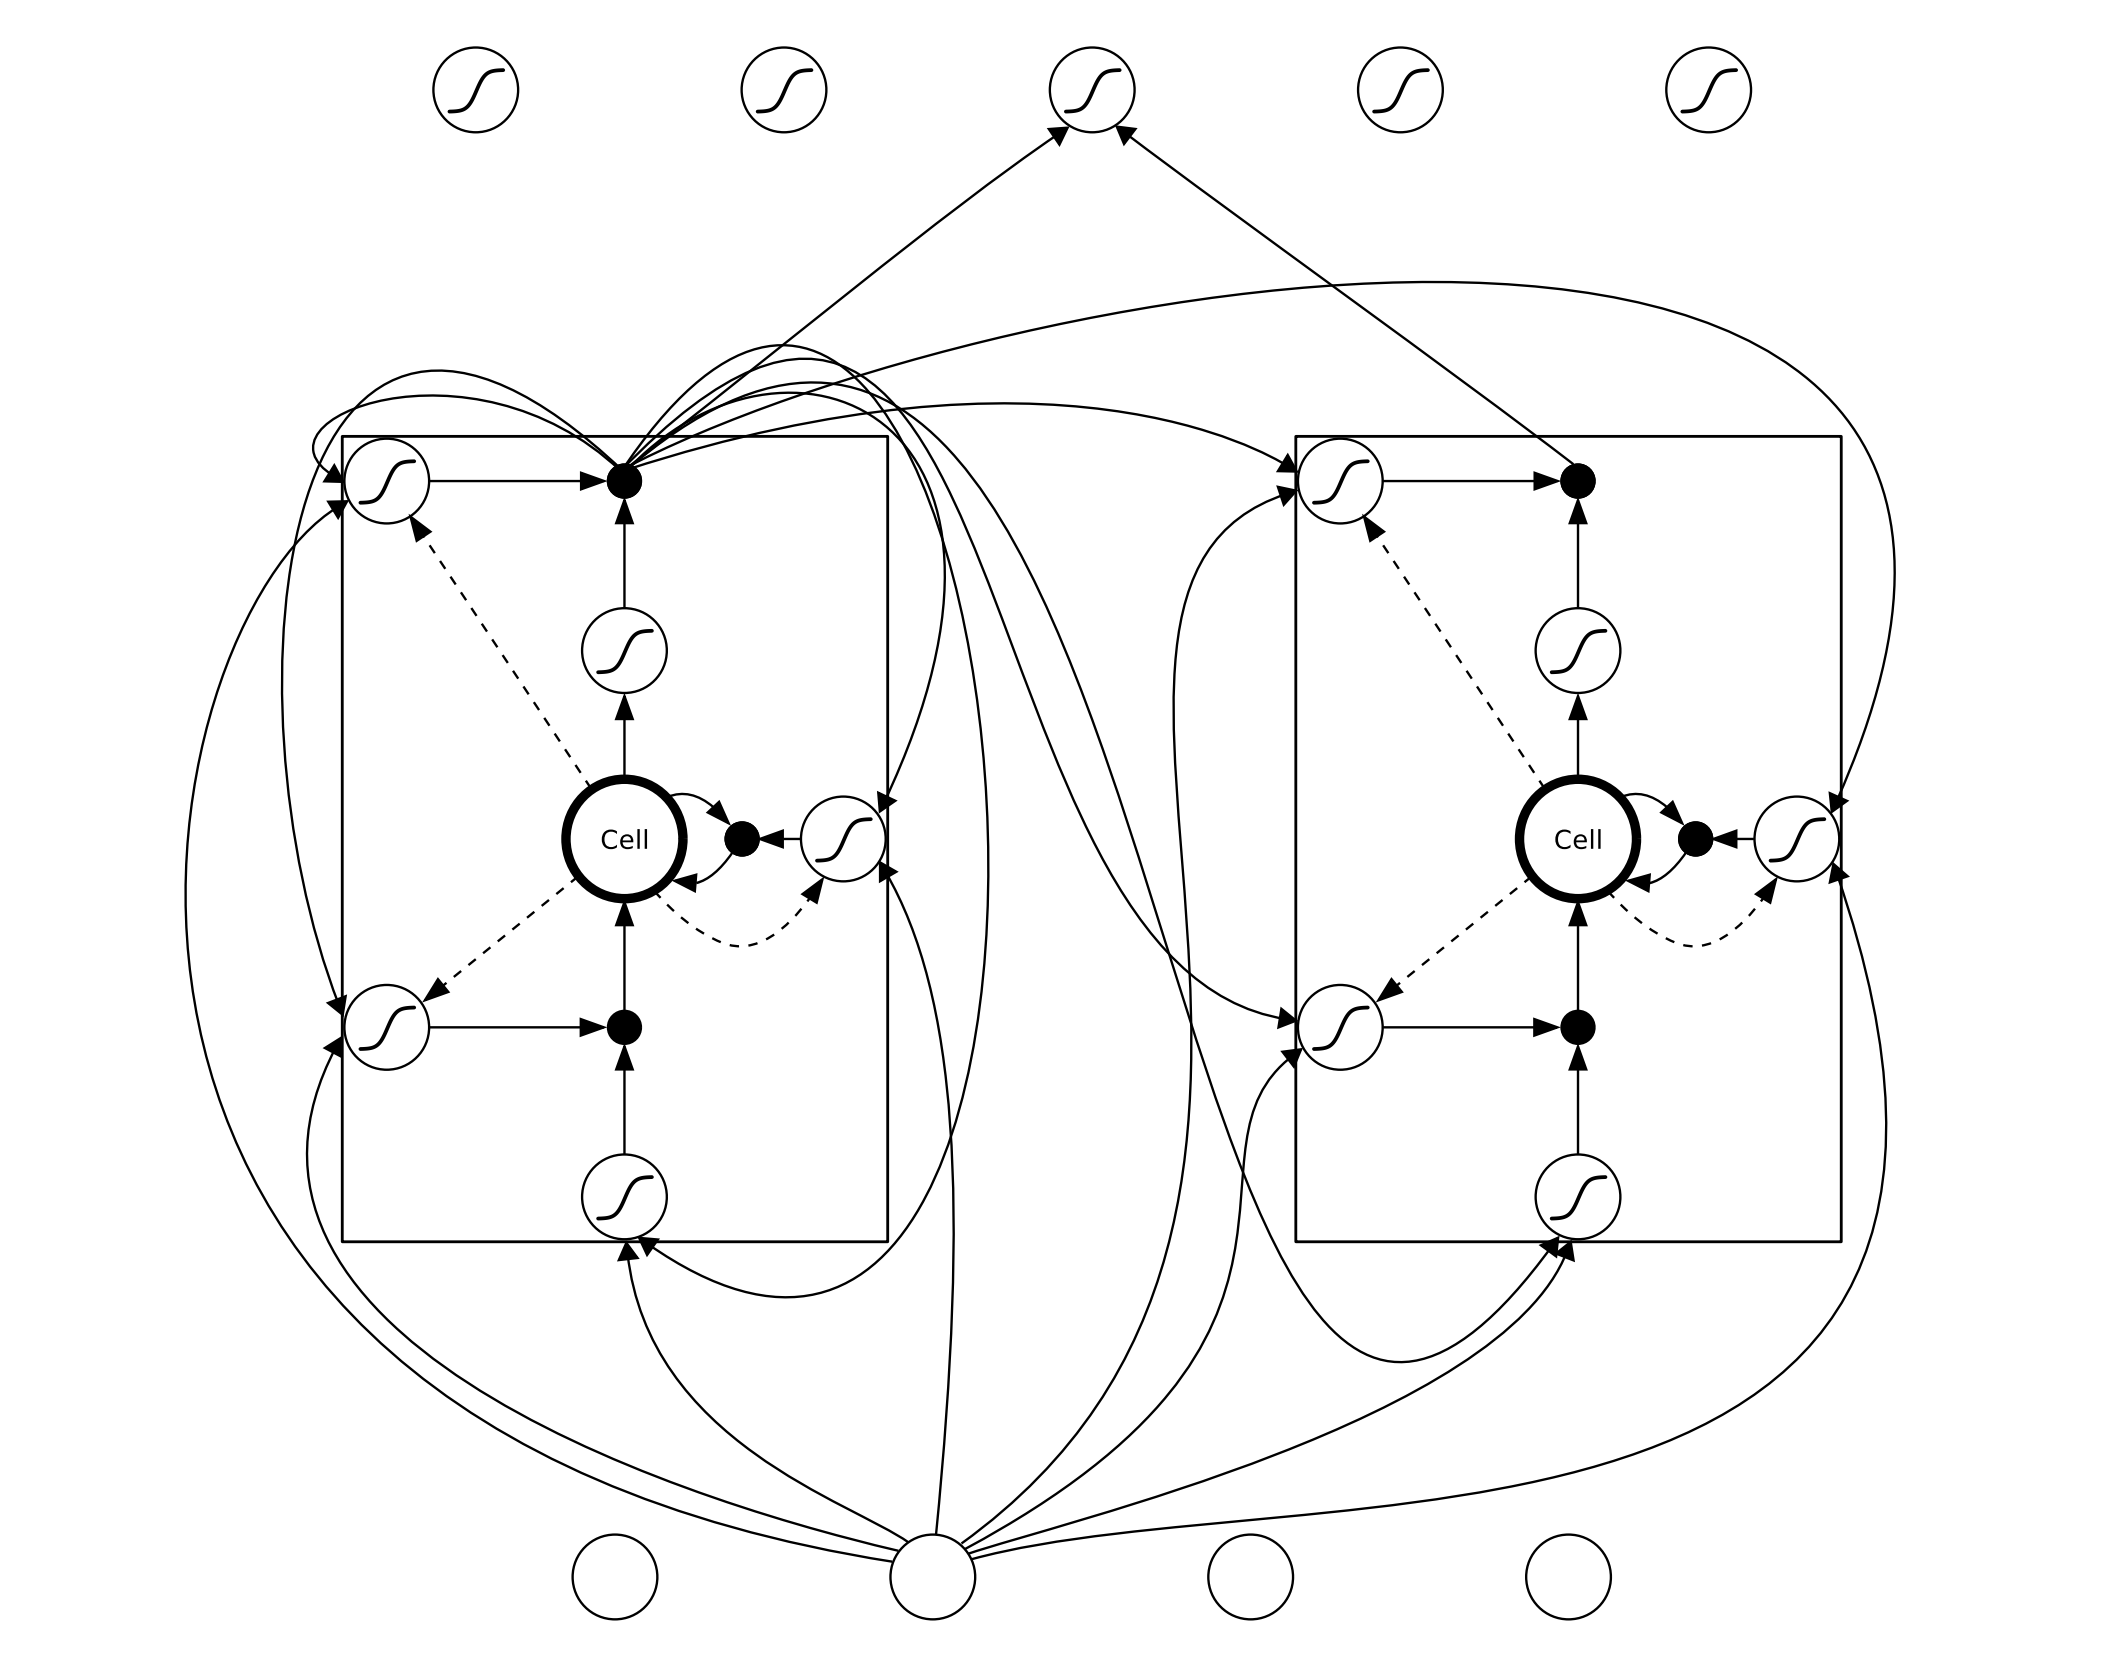
\includegraphics[width=9cm]{img/LSTM.png}
	\caption{An LSTM network.The network consists of four input units, a hidden layer of two single-cell LSTM memory blocks and five output units. Not all connections are shown. Note that each block has four inputs but only one output.}
	\label{LSTM}
\end{figure}

LSTM has been applied to various real-world problems, such
as protein secondary structure prediction \cite{hochreiter2007fast} \cite{chen2005protein}, music generation \cite{eck2002finding}, reinforcement learning \cite{bakker2002reinforcement}, speech recognition \cite{graves2005framewise} \cite{graves2006connectionist} and handwriting recognition \cite{graves2009offline} \cite{graves2008unconstrained}. As would be expected, its advantages are most pronounced for problems requiring the use of long range contextual information.

\subsection{Siamese neural network}
Siamese neural network \cite{bromley1994signature}, Figure \ref{siamese_fig}, consists of two identical sub-networks with shared weights joined at their outputs. This network has two input fields to compare two patterns and one output whose state value corresponds to the similarity between the two patterns.

\begin{figure}
	\centering
	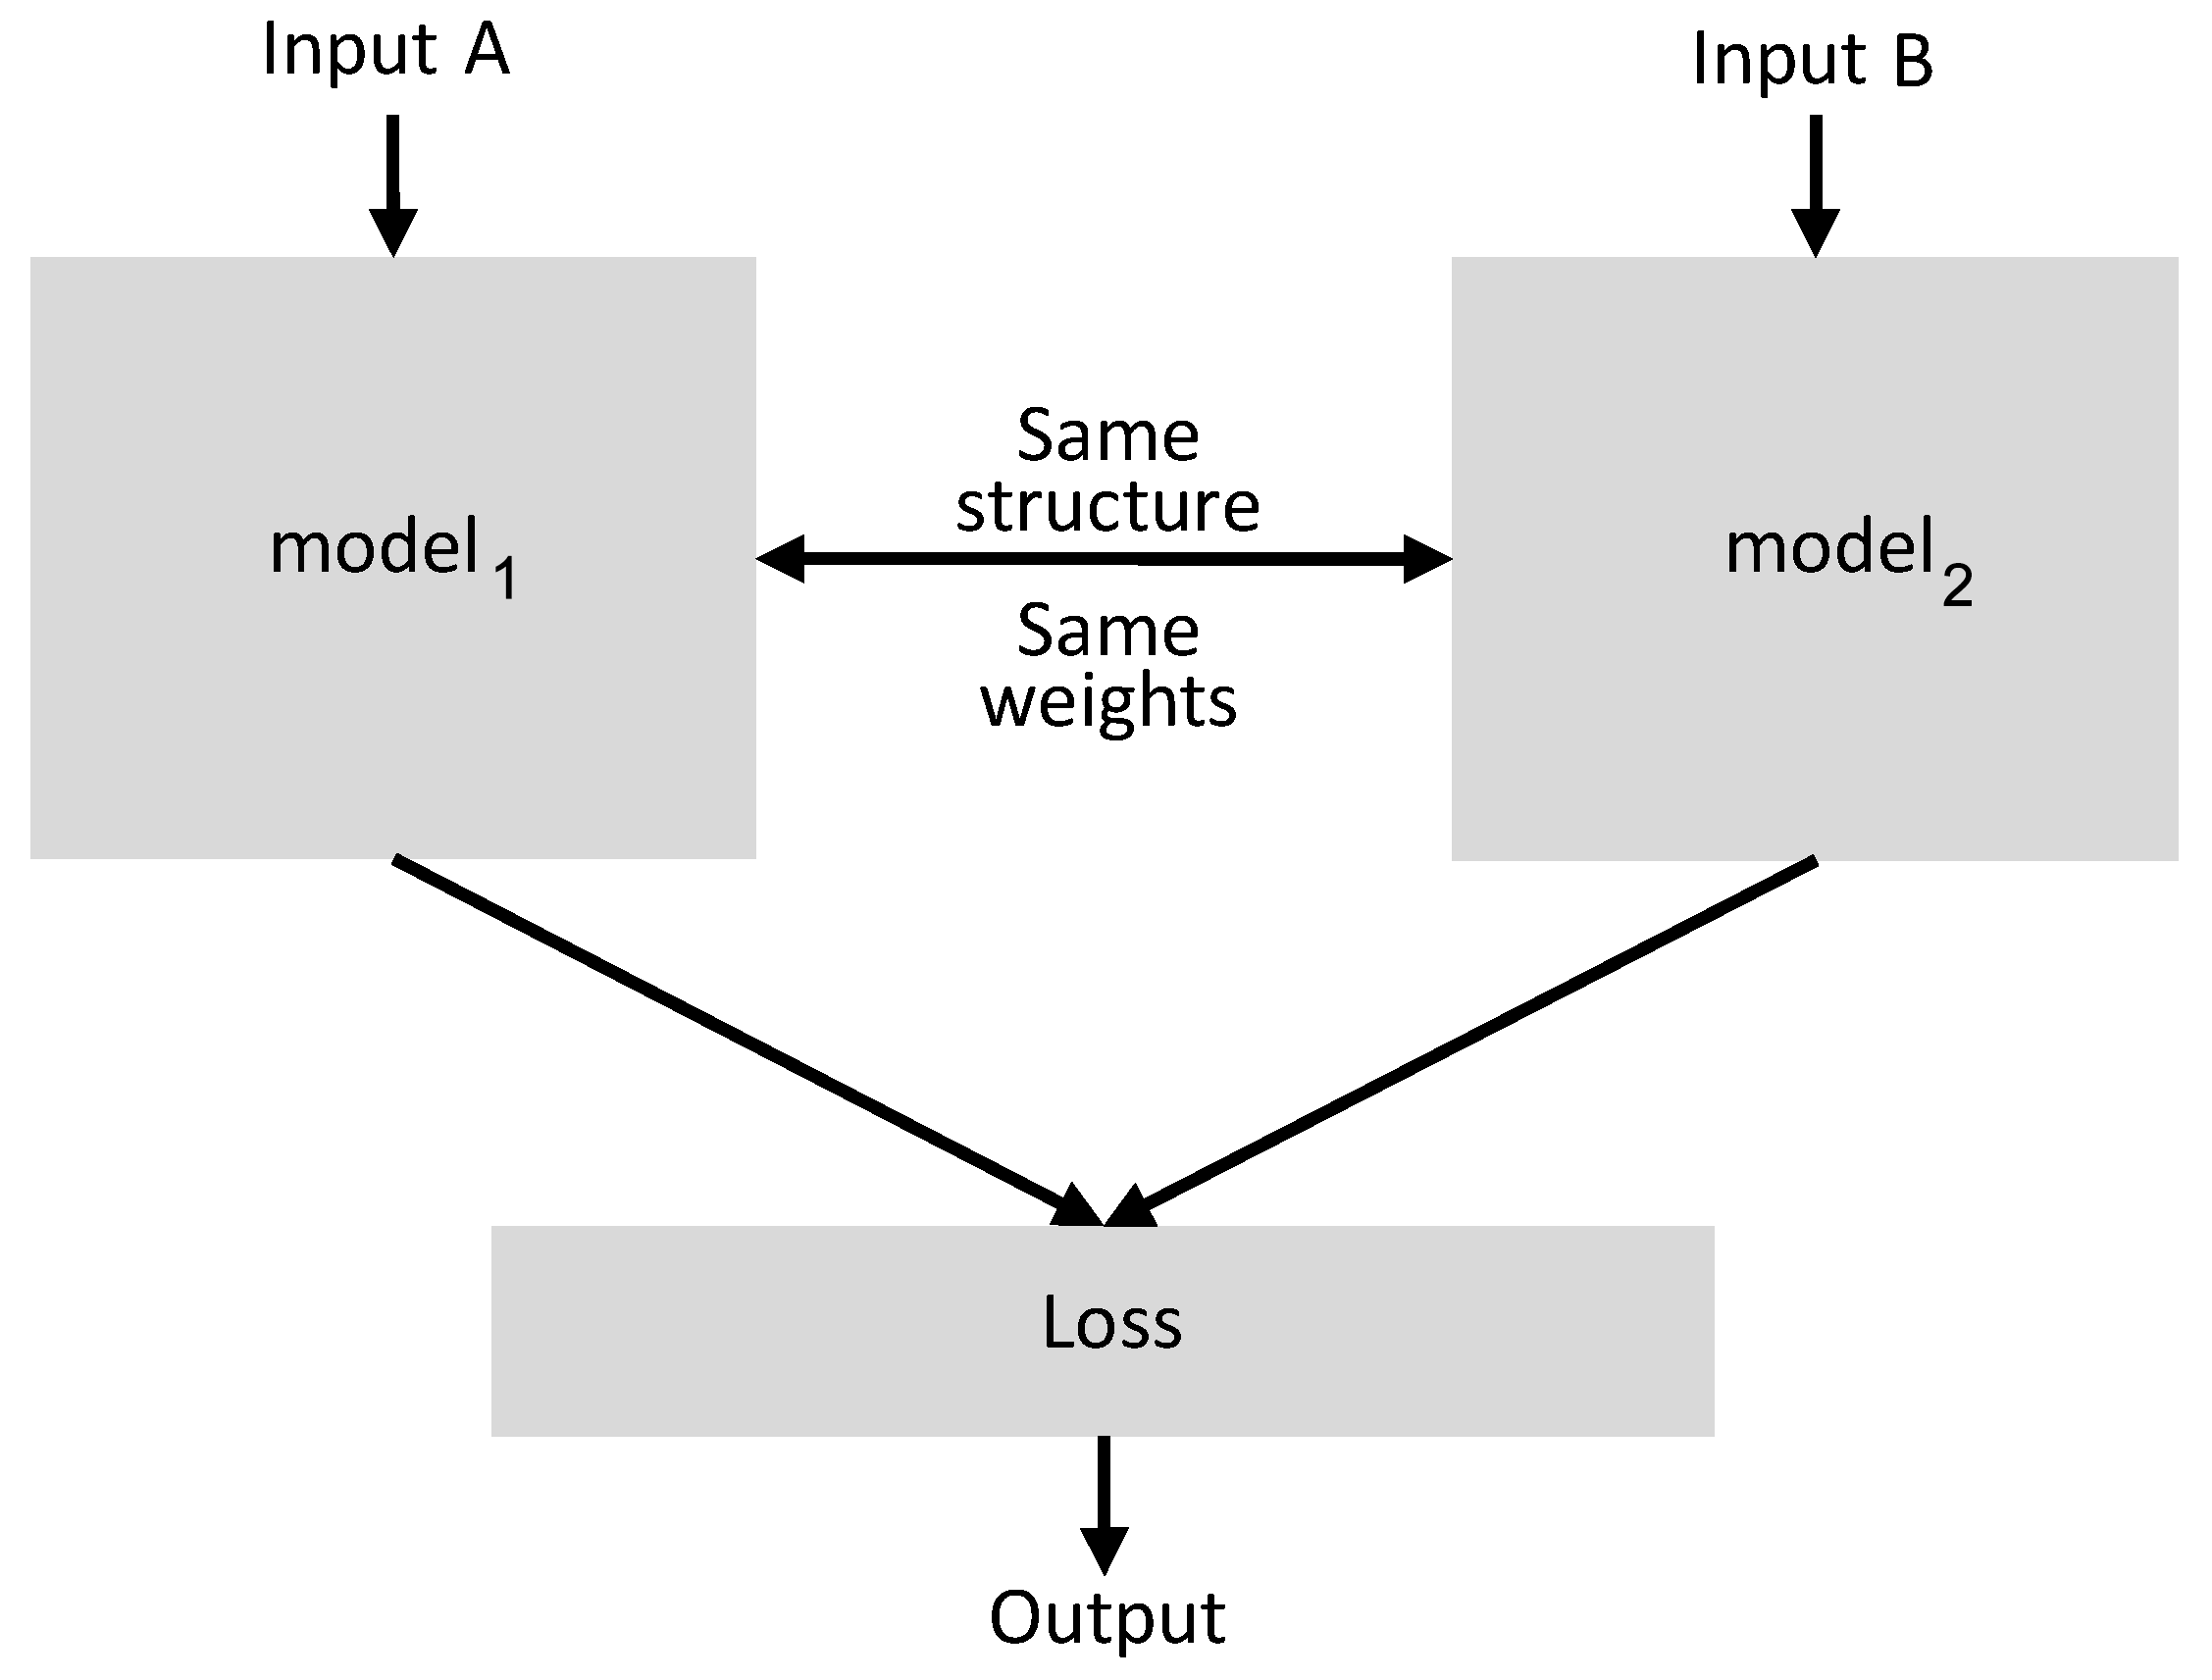
\includegraphics[width=10cm]{img/siamese.png}
	\caption{A generic Siamese neural network. The architecture is composed of the two identical models with shared weights that have different data input. The predictions are then evaluated by a loss function (e.g. Margin ranking loss).}
	\label{siamese_fig}
\end{figure}

The last layer compares the output of the two identical sub-networks and forces the distance, for example, of same category images to be 0 and 1 for the different ones. A contrastive loss function is used for this purpose, which was introduced by Yann LeCun \cite{hadsell2006dimensionality}:

\begin{equation}
L(W, Y, \overrightarrow{X1}, \overrightarrow{X2})=(1-Y)\frac{1}{2}(D_{W})^2 +(Y)\frac{1}{2}\{\max{(0,m-D}_{W})\}^2
\end{equation}

where $Dw$ is the distance output by the network, $Y$ the real value (0/1) and m a parameter which value is determined by the maximum distance chosen (1).
Other loss functions to train the Siamese neural networks are triplet loss \cite{triplet_loss} and Margin ranking loss \cite{rankingloss}. In particular Margin ranking loss was used for the proposed model.